\documentclass{beamer}
\usepackage{stmaryrd}
\usepackage{galois}
\usepackage{bussproofs}
\usepackage{tikz}
\usepackage{bbm}
\newcommand{\bind}{\gg\!\!=}

% Macros {{{
\newcommand{\kw}[1]{\ensuremath{ \mathsf{#1} }}
\newcommand{\ifr}[1]{\ [{#1}]\ }
\newcommand{\ifrw}[2]{\ [{#1}]_{#2}\ }

\newcommand{\EC}{\kw{C}}
\newcommand{\simrel}{\kw{simrel}}
%}}}

\AtBeginSection[]
{
   \begin{frame}
        \tableofcontents[currentsection]
   \end{frame}
}

\title{Refinement-Based Game Semantics for CompCert}
\author{\underline{J\'er\'emie Koenig} \and Zhong Shao}

\begin{document}

\maketitle

\section{Introduction} %{{{

\begin{frame}{Goal} %{{{

Tension:
\begin{itemize}
\item
  To make verification tractable,
  we need semantic models that are
  specialized to the task at hand.
\item 
  To link verified artefacts together and
  build large-scale certified systems,
  we need compatible semantic models.
\end{itemize}
\vfill

Our hope:
\begin{itemize}
\item
  To build a general-purpose, compositional
  semantic model supporting large-scale reasoning
  about heterogenous systems.
\item
  To enable linking disparate verification projects
  by making sure more specialized semantics
  can be embedded into ours.
\end{itemize}
\vfill

\end{frame}
%}}}

\begin{frame}{Building Certified Systems} %{{{
\small
\begin{center}
  \fbox{%
    system description $\quad p \in P
    \quad \xrightarrow{\llbracket - \rrbracket} \quad
    \sigma \in \mathbb{D} \quad$ mathematical theory}
\end{center}
\begin{itemize}
\item \textbf{Refinement}
  \[ (\mathbb{D}, {\sqsubseteq}, {\sqcup}, {\sqcap})
     \mbox{ is a complete lattice} \]
\item \textbf{Compositionality}
  \begin{gather*}
    \llbracket p_1 + p_2 \rrbracket =
    \llbracket p_1 \rrbracket \oplus \llbracket p_2 \rrbracket
    \\
    \sigma_1 \sqsubseteq \sigma_1' \:\wedge\:
    \sigma_2 \sqsubseteq \sigma_2' \:\Rightarrow\:
    \sigma_1 \oplus \sigma_2 \sqsubseteq \sigma_1' \oplus \sigma_2'
  \end{gather*}
\item \textbf{Abstraction}
  \begin{gather*}
    (\mathbb{D}^\natural, {\sqsubseteq})
    \galois{\alpha}{\gamma}
    (\mathbb{D}^\sharp, {\sqsubseteq})
    \\
    \alpha(\sigma^\natural) \sqsubseteq \sigma^\sharp
    \: \Leftrightarrow \:
    \sigma^\natural \sqsubseteq_\mathbb{C} \sigma^\sharp
    \: \Leftrightarrow \:
    \sigma^\natural \sqsubseteq \gamma(\sigma^\sharp)
  \end{gather*}
\end{itemize}
\end{frame}
%}}}

%\begin{frame}{Candidates} %{{{
%\begin{center}
%  \begin{tabular}{lcccc}
%                 & V & H & Abstraction & \ldots \\
%    CompCert LTS & $\bullet$ &   & &  \\
%    CAL & $\bullet$ & & $\bullet$ & \\
%    Interaction Semantics & $\bullet$ & $\bullet$ & & \\
%    I-Trees & $\bullet$ & $\bullet$ & ? & \\
%    R-B Game Semantics & $\bullet$ & $\bullet$ & $\bullet$ & $\bullet$ \\
%  \end{tabular}
%\end{center}
%\end{frame}
%%}}}

\begin{frame}{Game Semantics} %{{{
Basic idea:
\begin{center}
  \begin{tabular}{lcc}
  \hline
   & Types & Terms \\
  \hline
  Denotational semantics & Objects & Morphisms \\
  \hspace{1em} Traditional & Domains & Continuous functions \\
  \hspace{1em} Game semantics & Games & Strategies \\
  \hline
  \end{tabular}
\end{center}

\vfill
Game semantics:
\begin{itemize}
\item
  are usually formulated as trace semantics,
  with a strong distinction between
  system vs. environment actions;
\item
  can characterize
  the interactive behavior of program components
  more precisely than
  usual domain-theoretic approaches,
  thanks to a strong operational flavor.
\end{itemize}
\vfill
\end{frame}
%}}}

\begin{frame}{Our model} %{{{

We use simple
\emph{elementary games}
of the form $G = \langle M_G^Q, M_G^A \rangle$,
which consist of
one \emph{question} $m \in M_G^Q$ and
one \emph{answer} $n \in M_G^A$.

\vspace{1ex}
Two elementary games
$A = \langle M, N \rangle$ and
$B = \langle Q, R \rangle$
can be combined to form
the composite game $A \rightarrow B$:
\begin{center}
  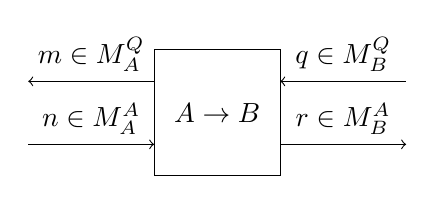
\begin{tikzpicture}[scale=0.4]
    \draw (-2, -2) rectangle (2, 2);
    \draw ( 2,  1) edge[<-] node[auto] {$q \in M_B^Q$} ( 6,  1);
    \draw ( 2, -1) edge[->] node[auto] {$r \in M_B^A$} ( 6, -1);
    \draw (-6,  1) edge[<-] node[auto] {$m \in M_A^Q$} (-2,  1);
    \draw (-6, -1) edge[->] node[auto] {$n \in M_A^A$} (-2, -1);
    \draw (0, 0) node {$A \rightarrow B$};
  \end{tikzpicture}
\end{center}

Traces for $A \rightarrow B$ are of the form:
\[
    q \, \mathbf{m} \, n \, \mathbf{m} \, n \cdots \mathbf{m} \, n \, \mathbf{r}
\]

$B$~specifies the \emph{incoming} questions
and the system's answers;
$A$~specifies \emph{outgoing}
questions and the environment's answers.
\end{frame}

\begin{frame}{Example: CompCert Open Modules}
CompCert C-style interactions
use the game:
\[ \mathcal{C} = \langle \{ f(\vec{v})@m \}, \, \{ v'@m' \} \rangle \]

Open modules will have type $\mathcal{C} \rightarrow \mathcal{C}$:
\begin{center}
  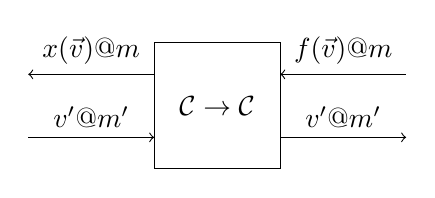
\begin{tikzpicture}[scale=0.4]
    \draw (-2, -2) rectangle (2, 2);
    \draw ( 2,  1) edge[<-] node[auto] {$f(\vec{v})@m$} ( 6,  1);
    \draw ( 2, -1) edge[->] node[auto] {$v'@m'$} ( 6, -1);
    \draw (-6,  1) edge[<-] node[auto] {$x(\vec{v})@m$} (-2,  1);
    \draw (-6, -1) edge[->] node[auto] {$v'@m'$} (-2, -1);
    \draw (0, 0) node {$\mathcal{C} \rightarrow \mathcal{C}$};
  \end{tikzpicture}
\end{center}

The codomain game specifies the form of incoming calls,
and the domain game specifies the form of external calls.
\end{frame}
%}}}

\begin{frame}{CompCert taxonomy} %{{{
Various flavors of CompCert can be classified according to
the game their semantics are playing:
\begin{center}
  \begin{tabular}{lc}
    \hline
    Variant & Semantic domain \\
    \hline
    CompCert  & $\ 1 \rightarrow \kw{int}$ \\
    CompCertX/CeritKOS & $1 \rightarrow \mathcal{C}$ \\
    Compositional CompCert & $\mathcal{C} \rightarrow \mathcal{C}$ \\
    This work & $A \rightarrow B$ \\
    \hline
  \end{tabular}
\end{center}

\vspace{1ex}
Where:
\begin{itemize}
\item $1 = \langle \varnothing, \varnothing \rangle$
  is the trivial game;
\item $\kw{int} = \langle \{*\}, \mathbb{B}^{32} \rangle$
  is the original interface of programs.
\end{itemize}
\end{frame}
%}}}

\begin{frame}{Our work} %{{{
We formalize a stategy model for the games $A \rightarrow B$ above
and modify CompCert to take advantage of this model.

\vspace{1em}
Our version is most similar to Compositional CompCert,
but uses:
\begin{itemize}
\item \emph{games} to specify
  the form of the interaction
  for each language;
\item \emph{simulation conventions} to
  establish a correpondance between the
  interactions of the source and target languages.
\end{itemize}

\vspace{1em}
Simulation conventions
characterizes the correctness proof of each pass
and their composition.
We use a \emph{logical relations} approach:
\begin{itemize}
\item \emph{CompCert KLRs} generalize memory injections and extensions;
\item \emph{parametricity theorems} establish properties of languages,
  and allow us to strengthen the proof to enable compositionality.
\end{itemize}

\end{frame}
%}}}

%}}}

\section{Semantic Model} %{{{

%\begin{frame}{Games} %{{{
%A game $A = \langle M_A^Q, M_A^A \rangle$ specifies:
%\begin{itemize}
%\item a set $M_A^Q$ of \emph{questions} (function invocations), and
%\item a set $M_A^A$ of \emph{answers} (corresponding returns).
%\end{itemize}
%
%\vfill
%For example, the game $\mathcal{C}$ has:
%\begin{itemize}
%\item questions of the form $m \in M_\mathcal{C}^Q ::= f/\sigma(\vec{v})@m$;
%\item answers of the form $n \in M_\mathcal{C}^A ::= v'@m'$.
%\end{itemize}
%
%\vfill
%A component of type $A \Rightarrow B$
%will accept incoming calls according to the game $B$ and
%may perform external calls according to the game $A$.
%For instance,
%Clight components have type
%$\mathcal{C} \Rightarrow \mathcal{C}$.
%\end{frame}
%%}}}

\begin{frame}{Language interfaces} %{{{
The games used in our development are:
\begin{center}
  \footnotesize
  \begin{tabular}{cllp{.5\textwidth}}
    \hline
    Name & Questions & Answers & Description \\
    \hline
    $\mathcal{C}$ & $f(\vec{v})@m$ & $v'@m'$ &
      C-style function calls (Clight--RTL) \\
    $\mathcal{L}$ & $f[\kw{ls}]@m$ & $\kw{ls}'@m'$ &
      Args. in abstract locations (LTL, Linear) \\
    $\mathcal{M}$ & $f[\kw{sp},\kw{ra},\kw{rs}]@m$ & $\kw{rs}'@m'$ &
      Args. via in-memory stack (Mach) \\
    $\mathcal{A}$ & $\kw{rs}@m$ & $\kw{rs}'@m'$ &
      Assembly-style control transfers (Asm) \\
    \hline
  \end{tabular}
\end{center}

\vspace{1em}
Specifically,
\begin{itemize}
\item the source semantics are of type $\mathcal{C} \rightarrow \mathcal{C}$ and
\item the target semantics are of type $\mathcal{A} \rightarrow \mathcal{A}$.
\end{itemize}
\end{frame}
%}}}

\begin{frame}{Language semantics} %{{{
We modify CompCert's transition systems
to account for interaction.

\vspace{1ex}
For the game $A \rightarrow B$,
we have
$L := \langle S, \rightarrow, I, X, Y, F \rangle$ where:
\begin{itemize}
\item $S$ is a set of states
\item ${\rightarrow} \subseteq S \times S$ is a transition relation;
\item $I \subseteq M_B^Q \times S$ specifies initial states;
\item $X \subseteq S \times M_A^Q$ identifies external calls;
\item $Y \subseteq S \times M_A^A \times S$ resumes the execution;
\item $F \subseteq S \times M_B^A$ specifies final states.
\end{itemize}

\vspace{1ex}
One execution might go:
\small
\[
  q \, I \, s \rightarrow \cdots \rightarrow
  s \, X \, \mathbf{m} \leadsto n \, Y \, s \rightarrow \cdots \rightarrow
  s \, X \, \mathbf{m} \leadsto n \, Y \, s \rightarrow \cdots \rightarrow
  s \, F \, \mathbf{r}
\]
\end{frame}
%}}}

\begin{frame}{Simulation conventions} %{{{
To relate interactions which happen in terms of different games,
we introduce \emph{simulation conventions}.

\vspace{1em}
For the source and target games $A_1$ and $A_2$,
a simulation convention
$\mathbb{R} = \langle W, R^Q, R^A \rangle$
specifies:
\begin{itemize}
\item a set of \emph{worlds} $W$;
\item a $W$-indexed relation
$R^Q \subseteq W \times M_{A_1}^Q \times M_{A_2}^Q$;
\item a $W$-indexed relation
$R^A \subseteq W \times M_{A_1}^A \times M_{A_2}^A$.
\end{itemize}

\vspace{1em}
We write $\mathbb{R} : A_1 \Leftrightarrow A_2$.
\end{frame}
%}}}

\begin{frame}{Simulations} %{{{
CompCert's forward and backward simulations are modified to
take these changes into account.
The simulations will have a type:
\[
  L_1 \le_{\mathbb{R}_A \Rightarrow \mathbb{R}_B} L_2 \qquad
  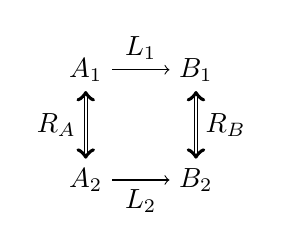
\begin{tikzpicture}[baseline,scale=0.7]
    \node (A1) at (-1,  1) {$A_1$};
    \node (A2) at (-1, -1) {$A_2$};
    \node (B1) at ( 1,  1) {$B_1$};
    \node (B2) at ( 1, -1) {$B_2$};
    \draw (A1) edge[->] node[auto] {$L_1$} (B1);
    \draw (A2) edge[->] node[auto,swap] {$L_2$} (B2);
    \draw (A1) edge[<->, double] node[auto,swap] {$\mathbb{R}_A$} (A2);
    \draw (B1) edge[<->, double] node[auto] {$\mathbb{R}_B$} (B2);
  \end{tikzpicture}
\]

The simulations add the following conditions:
\begin{itemize}
\item If the initial questions were related at a world $w \in W_B$,
  then the final answers must be related at that same world.
\item For each external call,
  there exists a world $v \in W_A$ that relates
  the source and target questions.
  The environment's answers must be related at that world
  for the simulation to resume.
\end{itemize}
\end{frame}
%}}}

\begin{frame}{Composition of simulations} %{{{
We can define the identity simulation convention $\mathbbm{1}$,
which is such that $L \le_{\mathbbm{1} \Rightarrow \mathbbm{1}} L$
for all transition systems $L : A \rightarrow B$.

\vspace{1em}
We can define the composite simulation convention
$\mathbb{R} \circ \mathbb{S} : A_1 \Leftrightarrow A_3$ for
$\mathbb{R} : A_1 \Leftrightarrow A_2$ and
$\mathbb{S} : A_2 \Leftrightarrow A_3$.
Simulations compose as expected:
\[
  \AxiomC{$L_1 \le_{\mathbb{R}_A \Rightarrow \mathbb{R}_B} L_2$}
  \AxiomC{$L_2 \le_{\mathbb{S}_A \Rightarrow \mathbb{S}_B} L_3$}
  \BinaryInfC{$L_1 \le_{\mathbb{R}_A \circ \mathbb{S}_A \Rightarrow \mathbb{R}_B \circ \mathbb{S}_B} L_3$}
  \DisplayProof
  \qquad
  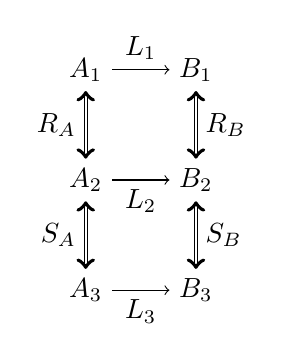
\begin{tikzpicture}[baseline,scale=0.7]
    \node (A1) at (-1,  2) {$A_1$};
    \node (A2) at (-1,  0) {$A_2$};
    \node (A3) at (-1, -2) {$A_3$};
    \node (B1) at ( 1,  2) {$B_1$};
    \node (B2) at ( 1,  0) {$B_2$};
    \node (B3) at ( 1, -2) {$B_3$};
    \draw (A1) edge[->] node[auto] {$L_1$} (B1);
    \draw (A2) edge[->] node[auto,swap] {$L_2$} (B2);
    \draw (A3) edge[->] node[auto,swap] {$L_3$} (B3);
    \draw (A1) edge[<->, double] node[auto,swap] {$\mathbb{R}_A$} (A2);
    \draw (B1) edge[<->, double] node[auto] {$\mathbb{R}_B$} (B2);
    \draw (A2) edge[<->, double] node[auto,swap] {$\mathbb{S}_A$} (A3);
    \draw (B2) edge[<->, double] node[auto] {$\mathbb{S}_B$} (B3);
  \end{tikzpicture}
\]
\end{frame}
%}}}

\begin{frame}{Our Approach to Compositional Correctness}



%}}}

\section{CompCert KLRs}

\begin{frame}{Logical relations and CompCert}
CompCert's memory model
is the algebraic structure at the core of
its language semantics.
Memory extension and injections
are instances of \emph{logical relations}
for that algebraic structure.

\vspace{1em}
CompCert's memory extensions and injection
can be understood as logical relations:
elementary operations are compatible with them,
and we can systematically build up more complex relations
and prove larger relational properties,
up to and including simulation diagrams.

\vspace{1em}
Injections additionally use a set of worlds (\texttt{meminj}),
and an accessibility relation (\texttt{inject\_incr})
to make sure pointers are related consistently throughout
the memory.
We generalize from there
to \emph{CompCert KLRs}.
\end{frame}

\begin{frame}{Example: Memory model operations}
  \begin{align*}
      \kw{Mem.alloc} :
        &\Vdash R^\kw{mem} \rightarrow {=} \rightarrow {=} \rightarrow
        \Diamond (R^\kw{mem} \times R^\kw{block})
      \\
      \kw{Mem.free} :
        &\Vdash R^\kw{mem} \rightarrow R^\kw{ptrrange} \rightarrow
        \kw{option}^\le(\Diamond R^\kw{mem})
      \\
      \kw{Mem.load} :
        &\Vdash R^\kw{mem} \rightarrow R^\kw{ptr} \rightarrow
        \kw{option}^\le(R^\kw{val})
      \\
      \kw{Mem.store} :
        &\Vdash R^\kw{mem} \rightarrow R^\kw{ptr} \rightarrow R^\kw{val} \rightarrow
        \kw{option}^\le(\Diamond R^\kw{mem})
      \\
      \kw{Mem.perm} :
        &\Vdash R^\kw{mem} \rightarrow R^\kw{ptr} \rightarrow {\subseteq}
  \end{align*}
\end{frame}

\begin{frame}{Relational parametricity}
From CKLRs, we can derive simulation conventions
for games such as $\mathcal{C}$.

\vspace{1em}
For example
we define $\mathcal{C}[R] : \mathcal{C} \Leftrightarrow \mathcal{C}$
as follows:
\[
    \mathcal{C}[R] := \langle
      W, \:
      ({=} \times {=} \times {R^\kw{val}}^* \times R^\kw{mem}), \:
      \Diamond (R^\kw{val} \times R^\kw{mem})
    \rangle \,.
\]
\end{frame}

\section{Compiler Correctness}

\begin{frame}{Notable CKLRs}
The CKLRs used in our development are:
\begin{itemize}
  \item \textbf{ext}: memory extensions (uses a trivial set of worlds)
  \item \textbf{inj}: memory injections (\texttt{meminj},
    \texttt{Mem.inject}, etc.)
  \item \textbf{injp}: injections + CompCert's external call requirements
\end{itemize}

\vspace{1ex}
They satisfy the following properties:
\[
  \mathcal{C}[\kw{inj}] \cdot \mathcal{C}[\kw{inj}] \equiv
  \mathcal{C}[\kw{ext}] \cdot \mathcal{C}[\kw{inj}] \equiv
  \mathcal{C}[\kw{inj}] \cdot \mathcal{C}[\kw{ext}] \equiv
  \mathcal{C}[\kw{inj}] \,.
\]

Using this infrastructure,
we do not need extensive changes to the existing CompCert proofs:
although individual passes are not symmetric in terms of their
requirements vs. guarantees,
we will be able to exploit languages properties
to reconcile them at the scale of the whole compiler.
\end{frame}

\begin{frame}{Passes}
\begin{center}
  \tiny
  \begin{tabular}{lllp{.55\textwidth}}
    \hline
    Language/Pass & Outgoing & Incoming & Description \\
    \hline
    \textbf{Clight} & $\mathcal{C}$ & $\mathcal{C}$ &
      A simpler version of CompCert C;
      expressions have no side-effects. \\
    \emph{Eqn.}~(\ref{eqn:clight}) & $\mathcal{C}[\kw{injp}]^*$ & $\mathcal{C}[\kw{injp}]^*$ &
      \emph{Clight properties} \\
    \kw{SimplLocals} & $\mathcal{C}[\kw{injp}]$ & $\mathcal{C}[\kw{inj}]$ &
      Pulling non-adressable scalar local variables out of memory. \\
    \kw{Cshmgen} & \kw{id} & \kw{id} &
      Simplification of control structures;
      explication of type-dependent computations. \\
    \hline
    \textbf{Csharpminor} & $\mathcal{C}$ & $\mathcal{C}$ &
      Low-level structured language. \\
    \kw{Cminorgen} & $\mathcal{C}[\kw{injp}]$ & $\mathcal{C}[\kw{inj}]$ &
      Stack allocation of local variables whose address is taken. \\
    \hline
    \textbf{Cminor} & $\mathcal{C}$ & $\mathcal{C}$ &
      Low-level structured language,
      with explicit stack allocation of certain local variables. \\
    \kw{Selection} & $\mathcal{C}[\kw{ext}]$ & $\mathcal{C}[\kw{ext}]$ &
      Recognition of operators and addressing modes. \\
    \hline
    \textbf{Cminorsel} & $\mathcal{C}$ & $\mathcal{C}$ &
      Like Cminor, with machine-specific operators and addressing modes. \\
    \kw{RTLgen} & $\mathcal{C}[\kw{ext}]$ & $\mathcal{C}[\kw{ext}]$ &
      Construction of the CFG, 3-address code generation. \\
    \hline
    \textbf{RTL} & $\mathcal{C}$ & $\mathcal{C}$ &
      Register transfer language. \\
    \kw{Tailcall} & $\mathcal{C}[\kw{ext}]$ & $\mathcal{C}[\kw{ext}]$ &
      Recognition of tail calls. \\
    \kw{Renumber} & $\kw{id}$ & $\kw{id}$ &
      Postorder renumbering of the CFG. \\
    \emph{Eqn.}~(\ref{eqn:rtl}) & $\mathcal{C}[\kw{inj}]$ & $\mathcal{C}[\kw{inj}]$ &
      \emph{RTL properties} \\
    \kw{Allocation} & \kw{alloc} & \kw{alloc} &
      Register allocation \\
    \hline
    \textbf{LTL} & $\mathcal{L}$ & $\mathcal{L}$ &
      Location transfer language. \\
    \kw{Linearize} & \kw{id} & \kw{id} &
      Linearization of the CFG \\
    \hline
    \textbf{Linear} & $\mathcal{L}$ & $\mathcal{L}$ &
      Like LTL, but the CFG is replaced by
      a linear list of instructions \\
    \kw{CleanupLabels} & \kw{id} & \kw{id} &
      Removal of unreferenced labels. \\
    \kw{Debugvar} & \kw{id} & \kw{id} &
      Synthesis of debugging information. \\
    \kw{Stacking} & \kw{stacking} & \kw{stacking} &
      Laying out the activation records \\
    \hline
    \textbf{Mach} & $\mathcal{M}$ & $\mathcal{M}$ &
      Like Linear, with a more concrete view of the activation record \\
    \kw{Asmgen} & \kw{asmgen} & \kw{asmgen} &
      Emission of assembly code \\
    \hline
    \textbf{Asm} & $\mathcal{A}$ & $\mathcal{A}$ &
      Assembly language for x86 machines \\
    \hline
  \end{tabular}
\end{center}
\end{frame}

\begin{frame}{Correctness theorem}
the overall simulation convention for the whole compiler
can be given as:
\[
  \mathbb{R}_\kw{CompCert} : \mathcal{C} \Leftrightarrow \mathcal{A} :=
    \mathcal{C}[\kw{injp}]^* \cdot
    \mathcal{C}[\kw{inj}] \cdot
    \kw{alloc} \cdot
    \kw{stacking} \cdot
    \kw{asmgen} \,.
\]

From the relational parametricity of Clight and RTL
and the properties outlined above we can show
that the composition of passes is compatible with
$\mathbb{R}_\kw{CompCert}$ on both sides and
conclude that if
$\kw{CompCert}(p_s) = p_t$
we have:
\[
      \kw{Clight} \llbracket p_s \rrbracket
      \le_{\mathbb{R}_\kw{CompCert} \Rightarrow \mathbb{R}_\kw{CompCert}}
      \kw{Asm} \llbracket p_t \rrbracket \,.
\]
\end{frame}

\section{Conclusion}

\begin{frame}{Conclusion}
\end{frame}

\end{document}
